% Chapter 2

\chapter{Scope} % Main chapter title
\label{Chapter2} % For referencing the chapter elsewhere, use \ref{Chapter2} 

%This chapter presents the scope of the thesis. The main work of this research 
%is to study the offline analysis of ScaRR's model.
%\ft{``Section~\ref{sec:implementation}'' is always capital letter, and add
%a tilde ``\textasciitilde'' in between.}
%In Section~\ref{sec:implementation}, we presents the scope of implementation. 
%Section
%\ref{sec:analysis} discusses the scope of the analysis.

%\section{Implementation}
%\label{sec:implementation}

%\begin{figure}[t]
%\centerline{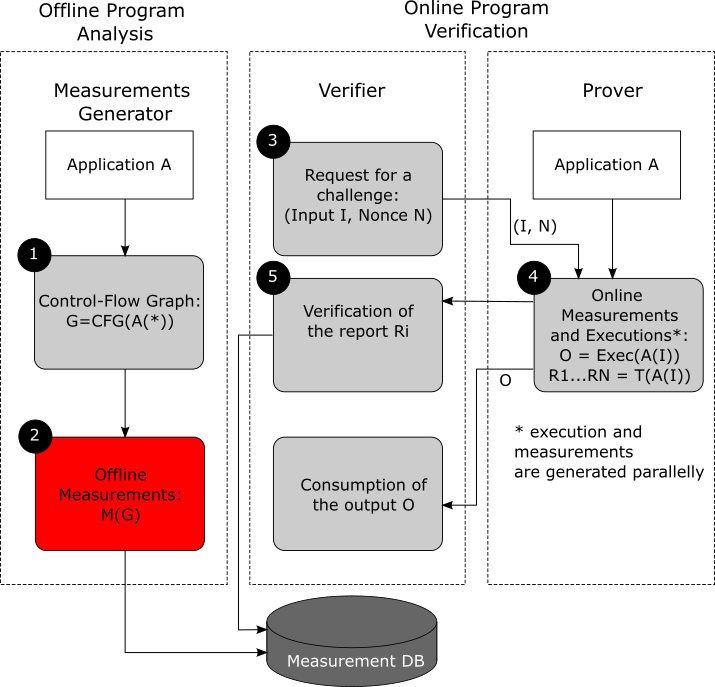
\includegraphics[scale=.5]{Figures/02/scarr-system-overview.png}}
%\caption{ScaRR System Overview}
%\label{fig:scarr-system-overview}
%\end{figure}

\ft{ALWAYS PRESENT!!! CHECK ALL THE TEXT}

%In Chapter \ref{Chapter1}, we presented different runtime remote attestation
%approaches. In learning the different models of runtime remote attestation, we
%implemented one of the model: 
The main work of this research is to study the offline analysis of ScaRR's 
model~\cite{toffaliniScaRRScalableRuntime2019} over a set of programs written 
in C \textbackslash C++. 
Specifically, we write a tool to extract offline measurement using the ScaRR 
control-flow model, verify the scalability of the algorithm, and study its 
limitation.

To sum up, the main contributions of this thesis are:
\begin{enumerate}
	\item propose an implementation of ScaRR's offline measurement extractor.
	\item verify the scalability of ScaRR's offline measurement algorithm.
	\item study the algorithm limitation.
\end{enumerate}
%ScaRR system as
%shown in figure \ref{fig:scarr-system-overview}, consists of offline program
%analysis and online program verification. 
%This thesis will focus on the offline program analysis, specifically on the 
%offline measurements generator as shown in the red box in the figure 
%\ref{fig:scarr-system-overview}.

% NO NEED THIS PART
%The offline measurement is information that will be used in runtime remote
%attesttion. We write the offline measurement as LLVM passes
%\cite{lattnerLLVMINFRASTRUCTUREMULTISTAGE2002} using LLVM 13.0.0. We designed
%the algorithm based on the description in the original paper. 


%We tested the model implementation using different programs that is written in
%C. Since the LLVM pass is running against the intermediate representation (IR),
%we should get consistent result on any programming language that compiles to 
%IR.

% NO NEED!
%\section{Analysis}
%\label{sec:analysis}
%
%We analyze the control-flow model extracted against different programs with
%various size and complexities. In this thesis, we are only analyzing program
%written in C. The analysis is comparing the program size with different
%measurements defined by the ScaRR control-flow model. We present the detail of
%the methodology in chapter \ref{Chapter4} and show the analysis result in
%chapter \ref{Chapter5}.

\section{Outline}
\label{sec:outline}

\ft{here, make a list about the content of the following chapter as a list. For 
instance:}

\vspace{0.5cm}
\noindent \textbf{Chapter~\ref{Chapter3}:} We discuss the background.

\vspace{0.5cm}
\noindent \textbf{Chapter~\ref{Chapter4}:} \dots